\chapter{GIT}
\TT{GIT} is a Version Control Software. GitHub, GitLab, GitBucket etc. are hosting repository services.
\TLi{Setting up GitLab}{./Code/GITLABsetup.txt}
\section{Setting up GIT}
\TLi{Setting up Git:}{./Code/GITsetup.txt}
%\BF{clone:}\\
\BF{Cloning:}\\
Clone just means to get a copy of the repository on the local machine.
\TLi{clone}{./Code/GITclone.txt}
\BF{Making a repo of an existing local folder:}\\
For existing local folders the procedure to get a remote repository is as follows. First the empty remote repository (project) \TT{origin/master} has to be created on the git-web-interface. Then the existing local folder is included via shell.
\TLi{remote add}{./Code/GITremoteadd.txt} 
In the file \TT{.gitignore} it can be specified which filse are to be ignored by git.
\TLi{}{./Code/GitIgnore.txt}
\section{GIT-Handling}
\TLi{GIT Manual}{./Code/GIThelp.txt}
%\BF{add-commit-push:}\\
Before a file or a folder can be committed it has to be moved to the staging area this is done with \TT{add}. The \TT{commit}-command saves the changes\footnote{\TT{commit} is like a save button, it saves a state to which one could fall back} together with a commit-hash. The \TT{push}-command pushes the files/folders in the staging area to \TT{origin} on \TT{master}, where\TT{origin} is the remote repository and \TT{master} is the current branch.  
\TLi{add commit push}{./Code/GITacp.txt}
%\BF{rm}
\TLi{rm}{./Code/GITrm.txt}
%\BF{log}
\TT{log} lists all the commits, with the commit message and the commit-hash.
\TLi{log}{./Code/GITlog.txt}

\TLi{diff}{./Code/GITdiff0.txt}
\TLi{diff example}{./Code/GITdiff1.txt}
\TLi{blame}{./Code/GITblame.txt}

\BF{pull:}\\
\TT{pull} up-dates the one's local repository.
\TLi{pull}{./Code/GITpull.txt}

\BF{Reset to a certain commit:}\\
\TT{--hard h1} sets the current branch back and rewrites the history of the branch, commits done after \TT{h1} will no longer be in the branch-history.\\
HEAD points to the current commit, so with \TT{git reset --soft HEAD@\{1\}} HEAD is set back, and the history is not lost.
\TLi{Reset}{./Code/GITreset0.txt}
Alternatively it can be branched of a certain commit see listing \ref{Branch of commit}.

\subsection{Conflicts}
User A pulls \TT{file.txt} from the repository. Then \TT{file.txt} gets changed in the repo by user B. On pushing \TT{file.txt} to the repo by user A a conflict can occur. \\
In order to resolve the conflict, user A has to pull the modified repo $\rightarrow$ the changes of A remain but the commits of B are included too. Conflicts are marked with \TT{<<<<<<<...>>>>>>>} and the respective commit-hash.
\TLi{file.txt with a conflict (after pull by A)}{./Code/file.txt}
Alternatively \TT{git -log} and \TT{diff} can be used in order to find the differences to the repo resp. the conflicts by hand.
\TLi{Differences to the repo}{./Code/GITconflictbyhand.txt}
\newpage
\subsection{Branches and Tags}
\TT{origin} is the remote repository and \TT{master} is the standard name for the main branch.
\begin{center}

\tikzset{
	Commit1/.pic={
        code={
\draw[black,fill=gray, opacity=0.7] (0,0) circle (0.08cm);
\draw[black,right](-0.02,0)node[rotate=90]{\tiny \texttt{commit}};
							}
	}
}

\tikzset{
	Merge/.pic={
        code={
\draw[black,fill=gray, opacity=0.9] (0,0) circle (0.08cm);
\draw[black,left](0,0)node[rotate=90]{\tiny \texttt{merge}};
							}
	}
}

\tikzset{
	Commit2/.pic={
        code={
\draw[black,fill=gray, opacity=0.7] (0,0) circle (0.08cm);
\draw[black,left](-0.02,0)node[rotate=90]{\tiny \texttt{commit}};
							}
	}
}


\tikzset{
	Tag1/.pic={
        code={
\draw[black](-0.15,0.2)rectangle(0.15,1.2);
\draw[black](0,0.7)node[rotate=90]{\tiny \texttt{Tag V1}};
\draw[black,fill=gray, opacity=0.7] (0,0) circle (0.08cm); 
							}
	}
}

\tikzset{
	Tag2/.pic={
        code={
\draw[black](-0.15,0.2)rectangle(0.15,1.2);
\draw[black](0,0.7)node[rotate=90]{\tiny \texttt{Tag V2}};
\draw[black,fill=gray, opacity=0.7] (0,0) circle (0.08cm); 
							}
	}
}


\tikzset{
	Tag3/.pic={
        code={
\draw[black](-0.15,-1.2)rectangle(0.15,-0.2);
\draw[black](0,-0.7)node[rotate=90]{\tiny \texttt{Tag V3}};
\draw[black,fill=gray, opacity=0.7] (0,0) circle (0.08cm); 
							}
	}
}


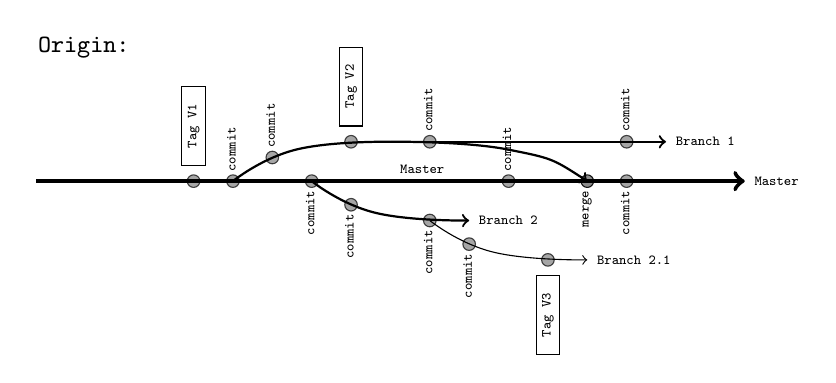
\begin{tikzpicture}
%Gitter
%\draw[step=0.5cm,very thin,black!20] (-6,-6) grid(6,6);
%\draw(-6,0)--(6,0);
%\draw(0,6)--(0,-6);

\path (-1.5,0.5) pic {Commit1};
\path (-0.5,0.5) pic {Commit2};
\path (1,1) pic {Commit1};



\path (3,0.5) pic {Merge};
\path (-2,0.5) pic {Tag1};
\path (2,0.5) pic {Commit1};
\path (3.5,1) pic {Commit1};
\path (3.5,0.5) pic {Commit2};

\path (-1,0.8) pic {Commit1};
\path (0,1) pic {Tag2};

\path (0,0.2) pic {Commit2};
\path (1,0) pic {Commit2};

\path (1.5,-0.3) pic {Commit2};
\path (2.5,-0.5) pic {Tag3};
\draw [black,ultra thick,->] plot [smooth, tension=0.8] coordinates {(-4,0.5) (5,0.5)};
\draw [black,->] plot [smooth, tension=0.8] coordinates {(1,0) (1.8,-0.4)(3,-0.5)};

\draw [black,thick] plot [smooth, tension=0.8] coordinates {(-1.5,0.5) (-0.7,0.9)(0.5,1)};

%\draw [black,thick,->] plot [smooth, tension=0.8] coordinates {(3,0.5) (3.8,0.9)(5,1)};
\draw [black,thick,->] plot [smooth, tension=0.8] coordinates {(0.5,1) (4,1)};


\draw [black,thick,<-] plot [smooth, tension=0.8] coordinates {(3,0.5) (2,0.9)(0.5,1)};


\draw [black,thick,->] plot [smooth, tension=0.8] coordinates {(-0.5,0.5) (0.3,0.1)(1.5,0)};

%\draw[black,right](0.5,1.15)node[rotate=00]{\tiny \texttt{Branch 1}};
\draw[black,right](4,1)node[rotate=00]{\tiny \texttt{Branch 1}};
\draw[black,right](0.5,0.65)node[rotate=00]{\tiny \texttt{Master}};
\draw[black,right](1.5,0)node[rotate=00]{\tiny \texttt{Branch 2}};
\draw[black,right](3,-0.5)node[rotate=00]{\tiny \texttt{Branch 2.1}};
\draw[black,right](5,0.5)node[rotate=00]{\tiny \texttt{Master}};
%\draw[black,right](4,0.5)node[rotate=00]{\small \texttt{Master}};
\draw[black,right](-4.1,2.2)node[rotate=00]{\small \texttt{Origin:}};
\end{tikzpicture}

\captionof{figure}[b]{Branches and Tags}
\end{center}

\subsubsection{Branching}
\TLi{Create Branch}{./Code/GITbranch.txt}
Branching of a certain commit.
\TLi{Create Branch of commit}{./Code/GITBranchofcommit.txt} 

\TT{branch -d} deletes a branch. After a branch is deleted its commits are still available.
\TLi{Delete Branch}{./Code/GITdelete.txt}

Depending on branch chosen by \TT{checkout} the local repo changes.
\TLi{Checkout a Branch}{./Code/GITcheckout.txt} 


\TT{Merge} takes all the commits (resp. all the changes) of the branch and puts them to current branch. After a merge the branch keeps in existence as an independent branch.


\TLi{Merge}{./Code/GITmerge.txt}

\newpage
\subsubsection{Tags}
Tags are similar to branches, they mark special points on the 'version-tree' releases, important backups etc.\footnote{Tags are displayed under \TT{Tags} (GitLab) or \TT{releases} (GitHub) on the remote repository}Lightweight tags are just special commits, annotated tags have a corresponding message and details about the tagger are saved.
\TLi{Create Tag}{./Code/GITtag0.txt}
\TLi{Create Tag from previous commit}{./Code/GITtag2.txt}
\TLi{Remove Tags}{./Code/GITtag1.txt}

Tags cannot be checked out. However a branch can be created from the tag, an this tag can be checked out.
\TLi{checkout from Tag}{./Code/GITtag3.txt}

%\TLi{Remove Tags}{./Code/GITtag2.txt}
\subsection{Forks}
Collaborators to a repository can make changes without issuing pull requests, others can contribute to the repo via pull-requests.\\
\ \\
A fork creates a new instance of a repository at the point where it currently is. The owner of the forked version can do with it whatever  he wants to. The forked version is not linked to the original version, only in the sense that the fork owner can issue pull-request. 
\TLi{fork}{./Code/GITfork.txt}




A pull-request is a request from fork-owner N with no rights, the original-owner R. N to R: \textit{I have a suggestion, would you like to pull from my repository?} R can grant or deny this suggestion. The pull-request is best done on the web-interface via the pull-request button.